\documentclass[11pt]{aghdpl}
% \documentclass[en,11pt]{aghdpl}  % praca w języku angielskim
\usepackage[polish]{babel}
%\usepackage[english]{babel}
\usepackage[utf8]{inputenc}

% dodatkowe pakiety
\usepackage{enumerate}
\usepackage{listings}
\lstloadlanguages{TeX}

\lstset{
  literate={ą}{{\k{a}}}1
           {ć}{{\'c}}1
           {ę}{{\k{e}}}1
           {ó}{{\'o}}1
           {ń}{{\'n}}1
           {ł}{{\l{}}}1
           {ś}{{\'s}}1
           {ź}{{\'z}}1
           {ż}{{\.z}}1
           {Ą}{{\k{A}}}1
           {Ć}{{\'C}}1
           {Ę}{{\k{E}}}1
           {Ó}{{\'O}}1
           {Ń}{{\'N}}1
           {Ł}{{\L{}}}1
           {Ś}{{\'S}}1
           {Ź}{{\'Z}}1
           {Ż}{{\.Z}}1
}

%---------------------------------------------------------------------------

\author{Piotr Borowiec}
\shortauthor{P. Borowiec}

\titlePL{Strumieniowanie adaptacyjne danych multimedialnych z wykorzystaniem standardu DASH-MPEG}
\titleEN{}

\shorttitlePL{Strumieniowanie adaptacyjne DASH-MPEG} 
\shorttitleEN{}

\thesistype{Praca dyplomowa magisterska}
%\thesistype{Master of Science Thesis}

\supervisor{dr inż. Łukasz Czekierda}
%\supervisor{Marcin Szpyrka PhD, DSc}

\degreeprogramme{Informatyka}
%\degreeprogramme{Computer Science}

\date{2014}

\department{Katedra Informatyki}
%\department{Department of Applied Computer Science}

\faculty{Wydział Informatyki, Elektroniki i Telekomunikacji}
%\faculty{Faculty of Electrical Engineering, Automatics, Computer Science and Biomedical Engineering}

\acknowledgements{Serdecznie dziękuję ...}


\setlength{\cftsecnumwidth}{10mm}

%---------------------------------------------------------------------------

\begin{document}

\titlepages

\tableofcontents
\clearpage

\chapter{Wprowadzenie}
\label{cha:rozdzial1}

\begin{itemize}
\item Cel pracy - skąd się wziął pomysł, dlaczego praca jest tworzona
\item Struktura - krótki opis dotyczący kolejnych rozdziałów
\item Zakres merytoryczny - ramy dla projektu
\item Wkład własny - krótki opis co się zrobiło i jak przebiegały prace.
\end{itemize}
\chapter{Zarys problemu}
\label{cha:rozdzial2}

\begin{itemize}
\item Pokazanie jak zmienne warunki w sieci wpływają na strumieniowanie
\item Wyjaśnienie na czym polegają problemy związane z implementacją gładkiego strumieniowania adaptacyjnego
\item Przedstawienie istniejących rozwiązań związanych ze strumieniowaniem adaptacyjnym (wtyczka do VLC, dodatek do Youtube, wtyczka do Internet Explorera)
\end{itemize}

\chapter{Przegląd istniejących rozwiązań}
\label{cha:rozdzial3}

\section{Wstęp}

Istnieje wiele podejść do zagadnienia jakim jest strumieniowanie danych. Najbardziej popularnym spośród opisywanych poniżej jest para protokołów: Real-time Transport Protocol~i RTP Control Protocol~\cite{RFC3550}. W niniejszym rozdziale opisane zostaną również protokoły: Datagram Congestion Control Protocol~\cite{RFC4340} oraz standard DASH-MPEG~\cite{ISO-IEC-DASH}. W każdym z powyższych przypadków zostną zaprezentowane metody kontroli przeciążenia sieci i punktów końcowych transmisji.

\section{TCP}

\section{Datagram Congestion Control Protocol}

Protokół DCCP należy do warstwy transportowej i wspiera dwukierunkowe połączenia typu punkt-punkt. Cechą charakterystyczną tego protokołu jest niezawodne nawiązywanie i zrywanie połączenia oraz negocjacja parametrów połączenia. Sama transmisja oparta jest na przesyłaniu datagramów bez potwierdzeń. DCCP posiada kilka mechanizmów kontroli przeciążeń.

Każdy ze wspieranych przez DCCP mechanizmów kontroli przeciążeń posiada identyfikator CCID (Congestion Control Identifier). W trakcie negocjacji parametrów połączenia stacje końcowe wymieniają posortowaną listę akceptowalnych CCID (od najbardziej pożądanego do najmniej pożądanego), a następnie wybierają mechanizm, którym będą posługiwać się w trakcie transmisji~\cite{RFC5762}. RFC standaryzuje dwa mechanizmy kontroli przeciążeń:
\begin{itemize}
  \item CCID 2 - TCP-like Congestion Control
  \item CCID 3 - TCP-Friendly Rate Control
\end{itemize}
Pozostałe numery CCID (0-1 oraz 4-255) pozostają do tej pory niewykorzystane.

Mechanizm TCP-like Congestion Control korzysta z AIMD (Additive Increase/Multiplicative Decrease). Jeżeli TCP wykorzystuje AIMD to po otrzymaniu każdej poprawnej wiadomości ACK od odbiorcy, nadawca powiększa wielkość \textit{cwnd} (wielkość okna) o $\frac{1}{cwnd}$. W razie utraty pakietów okno jest pomniejszane dwukrotnie~\cite{Stevens}. Omawiany mechanizm zachowuje także liczniki czasu znane z TCP oraz algorytm powolnego startu~\cite{RFC2581}. TCP-like Congestion Control powinno być wykorzystywane przez aplikacje w których bardziej preferowane jest maksymalne wykorzystanie łącza od utrzymania stabilnego pasma (np. transfer plików)~\cite{RFC4341}.

TCP-Friendly Rate Control jest mechanizmem uznawanym za niezachłanny przy dzieleniu łącza z innymi strumieniami o charakterze TCP. Niezachłanność tego mechanizmu oznacza, że wykorzystuje on przepustowość nie większą niż dwukrotna wartość przepustowości, która zostałaby wykorzystana przez TCP w tych samych warunkach. TCP-Friendly Rate Control charakteryzuje się także dużo mniejszą zmiennością wartości przepustowości w czasie w porównaniu do TCP, co sprzyja zastosowaniu DCCP z CCID 3 w strumieniowaniu danych multimedialnych. `Wygładzenie' przepustowości transmisji jest okupione wolniejszą niż w TCP szybkością przystosowywania się strumienia do zmian w dostępnym paśmie~\cite{RFC5348}.


\begin{figure}[h!]
	\centering
		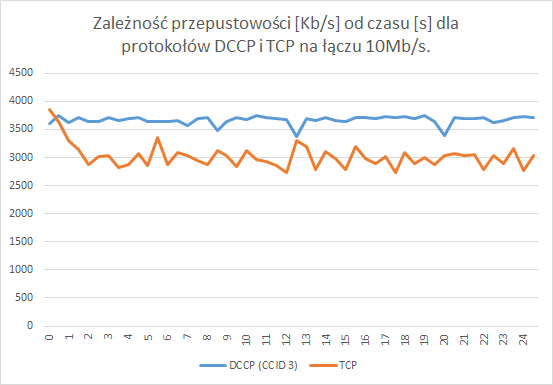
\includegraphics{TCP_DCCP}
	\caption{Wykres zależności przepustowości od czasu dla protokołów TCP i DCCP.}
	\label{TCP_DCCP}
\end{figure}

Rysunek~\ref{TCP_DCCP} przedstawia porównanie działania protokołów TCP i DCCP (CCID 3). W trakcie testu wykorzystano oprogramowanie D-ITG (Distributed Internet Traffic Generator)~\cite{D-ITG}. Test został przeprowadzony z wykorzystaniem dwóch komputerów i przełącznicy Cisco Catalyst 3550 połączonych w w jedną sieć LAN i polegał na jednoczesnym uruchomieniu dwóch strumieni (TCP i DCCP) pomiędzy stacjami końcowymi. Probkowanie przepustowości przeprowadzono co $0,5s$. Na przełącznicy zaimplementowano politykę pozwalającą na ustalenie przepustowości pomiędzy stacjami na 10Mb/s (zob. Dodatek A).

\begin{figure}[h!]
	\centering
	\begin{tabular}{ l | c | r }
  		Protokół & Średnia przepustowość & Odchylenie Standardowe \\
  		\hline
  		TCP & 2016 Kb/s & 206 \\
  		DCCP (CCID 3) & 2665 Kb/s & 74 \\
	\end{tabular}
	\caption{Tabela porównawcza protokołów TCP i DCCP.}
	\label{TCP_DCCP_table}
\end{figure}

Tabela z rysunku~\ref{TCP_DCCP_table} przedstawia porównanie średniej przepustowości~i ochylenia standardowego dla protokołów TCP i DCCP. Przeprowadzony test potwierdza zachowanie się protokołu DCCP (CCID~3) opisane w RFC 5348~\cite{RFC5348}. 

\section{Real-time Transport Protocol i RTP Control Protocol}

RTP (Real-time Transport Protocol) pozwala na transport danych w systemach i aplikacjach czasu rzeczywistego wspierających interaktywne transmisje audio i video. Zwykle wykorzystuje UDP jako protokół transportowy, ale może działać nad innymi protokołami warstwy transportowej modelu ISO/OSI (DCCP, TCP - \cite{RFC3550, RFC5762}). Jeżeli sieć w której działa RTP wspiera multicasting to RTP pozwala na wysłanie danych do wielu odbiorców jednocześnie. RTP nie dostarcza mechanizmów QoS (Quality of Service), ani nie gwarantuje dostarczenia wysłanych danych na czas do odbiorcy.

Protokół RTCP (Real-time Control Protocol) stanowi protokół kontrolny dla RTP. Bazuje na okresowej transmisji pakietów kontrolnych do wszystskich uczestników sesji. Przekazuje informacje od odbiorców do nadawców na temat jakości transmisji. Pakiety RTCP zawierają indentyfikator źródła (Canonical Name) oraz pozwalają na ustalenie liczby uczestników sesji, co pozwala na obliczenie z jaką częstotliwością należy wysyłać pakiety kontrolne.

\begin{figure}[h!]
	\centering
	\begin{tabular}{ l | c | r }
  		Nazwa & Typ & Zalecane pasmo \\
  		\hline
  		GSM & audio & 13 Kb/s \\
  		G728 & audio & 16 Kb/s  \\
  		G729 & audio & 8 Kb/s  \\
	\end{tabular}
	\caption{Przykładowe typy pakietów RTP.}
	\label{RTP_table}
\end{figure}

RTP przenosi dane, które zwykle wymagają ustalonej przepustowości. Dzięki temu prawdopodobieństwo, że strumień RTP będzie systematycznie zajmował coraz większe pasmo jest niewielkie. Z drugiej strony, strumień nie może też zostać ograniczony bez uszczerbku na jakości transmisji danych, szczególnie jeżeli transmisja ma charakter interaktywny. Pasmo potrzebne do sprawnej transmisji zależy od rodzaju przesyłanych danych. Rodzaj przesyłanych danych można identyfikować na podstawie pola Payload Type (zob. rysunek~\ref{RTP_table}) w nagłówku pakietu RTP. Z każdym typem związany jest profil RTP opisujący parametry transmisji (w tym wymaganą przepustowość)~\cite{RFC3551}. Protokół RTP nie posiada odpowiednich mechanizmów kontroli przeciążeń, dlatego powinien korzystać z mechanizmów dostępnych w protokołach niższych warstw (np. DCCP CCID 3).

\section{Dynamic Adaptive Streaming over HTTP}

Dynamic Adaptive Streaming over HTTP (DASH) jest adaptacyjną techniką strumieniowania danych przez Internet. DASH został opracowany przez grupę MPEG i stał się standardem w kwietniu 2012 dzięki publikacji ISO/IEC 23009-1:2012~\cite{ISO-IEC-DASH}. W lipcu 2013 wprowadzono poprawki do standardu.

DASH jest technologią spokrewnioną z Microsoft Smooth Streaming~\cite{MicroS}, Adobe Systems HTTP Dynamic Streaming~\cite{ADOBES} oraz Apple Inc. HTTP Live Streaming~\cite{APPLES}.

\begin{figure}[h!]
	\centering
		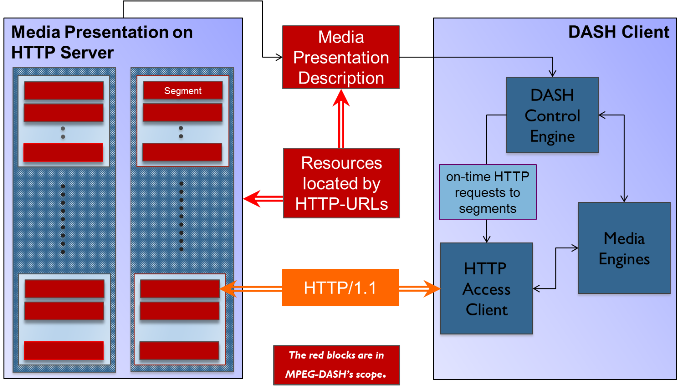
\includegraphics{dash}
	\caption{Standard MPEG-DASH i przykładowa architektura klienta DASH, źródło:~\cite{DASH}}
	\label{dash}
\end{figure}

W podejściu stosowanym w standardzie DASH logika strumieniowania zostaje w całości przeniesiona na aplikację klienta. Rolę serwera DASH może pełnić zwykły serwer plików. Plik multimedialny, który będzie podlegał operacji strumieniowania, należy odpowiednio przygotować. Plik powinien być dostępny w kilku wersjach różniących się jakością (a co za tym idzie również wielkością).  Każda kopia powinna zostać podzielona na segmenty o równej długości. Na rysunku~\ref{dash}~kopie pliku multimedialnego składają się z segmentów (czerwone prostokąty) umieszczonych na serwerze HTTP (lewa strona rysunku). Od długości segmentów zależeć będzie szybkość przystosowywania się aplikacji DASH do zmieniającej się przepustowości sieci. Tak przygotowane pliki należy opisać za pomocą xml w postaci dokumentu MPD (Media Presentation Description). Plik MPD zawiera adresy URL poszczególnych segmentów, informacje na teamt kodowania danych, rozdzielczości oraz wymaganych przepustowości. Następnie MPD musi zostać dostarczony klientowi, który parsując jego zawartość otrzyma informacje na temat pliku multimedialnego, który ma strumieniować. W trakcie strumieniowania, aplikacja klienta wybiera w sposób dynamiczny wersjię pliku i pobiera kolejny segment z pomocą protokołu HTTP. 

Standard DASH działa niezależnie od sposobu kodowania danych i jest łatwo implementowalny w Internecie. Dzięki wykorzystaniu protokołu HTTP może współpracować z istniejącą infrastrukturą w postaci filtrów, zapór, NAT'ów i cache'ów~\cite{DASH}.

\section{Podsumowanie}

W powyższym rozdziale opisano kilka podejść do problemu strumieniowania danych multimedialnych. Opisane zostały protokoły TCP, DCCP, RTP/RTCP oraz standard DASH-MPEG. Szczególną uwagę poświęcono mechanizmom adaptacji do zmniennej przepustowości sieci i cechom jakie powinny posiadać protokoły przeznaczone do strumieniowania danych. Do cech tych należą:
\begin{itemize}
\item kontrola przeciążeń i przepływu (TCP)
\item jednostajne wykorzystanie łącza (DCCP CCID3)
\item kanał zwrotny przenoszący informacje na temat sesji (RTCP)
\item możliwość dostosowana parametrów transmisji do warunków w sieci (DASH, TCP)
\end{itemize}


\chapter{Opis projektu i implementacji}
\label{cha:rozdzial4}


\chapter{Opis projektu i implementacji}
\label{cha:rozdzial5}

\begin{itemize}
\item Krótka prezentacja algorytmu zaimplementowanego z artykułu 
\item Prezentacja własnego algorytmu lub poprawek do algorytmu z punktu poprzedniego
\item Opis implemententacji programu klienta (diagram klas, sekwencji...)
\item Przedstawienie ewentualnych problemów przy implementacji i zastosowanych rozwiązań
\end{itemize}

\section{Opis algorytmu}

\section{Implementacja}

\section{Problemy i rozwiązania}
\chapter{Wdrożenie i testy}
\label{cha:rozdzial6}

\begin{itemize}
\item Opis instalacji i uruchamiania programu klienta
\item Opis przeprowadzonych testów działania/testów porównawczych
\item Pokazanie w jaki sposób skonfigurować sieć lokalną (multicasty) w celu zmniejszenia jej obciążenia przy transmisjach jeden-do-wielu. Tylko klient DASH łączy się do serwera. Pozostałe komputery w sieci kampusowej odbierają transmisję od klienta DASH.
\begin{center}
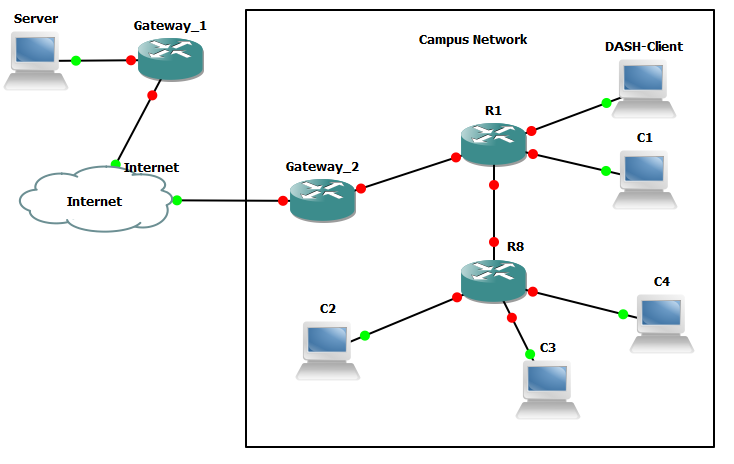
\includegraphics[scale=0.7]{lan}
\end{center}
\end{itemize}


\appendix
\chapter{Konfiguracja przełącznicy}
\label{cha:dodatekA}

Poniżej znajduje się konfiguracja przełącznicy wykorzystywanej do testów. Pominięta została konfiguracja interfejsów FastEthernet 3-24 oraz interfejsów GigabitEthernet.

\begin{verbatim}
!
version 12.2
no service pad
service timestamps debug uptime
service timestamps log uptime
no service password-encryption
!
hostname Switch
!
!
no aaa new-model
ip subnet-zero
!
mls qos aggregate-policer aggpolicer 10000000 8000 exceed-action drop
mls qos
!
no file verify auto
spanning-tree mode pvst
spanning-tree extend system-id
!
!
!
vlan internal allocation policy ascending
!
class-map match-all tcpmap
  match access-group 145
!
!
policy-map test
  class tcpmap
    police aggregate aggpolicer
!
!
!
interface FastEthernet0/1
 switchport mode dynamic desirable
 service-policy input test
!
interface FastEthernet0/2
 switchport mode dynamic desirable
 service-policy input test
!
interface Vlan1
 no ip address
 shutdown
!
ip classless
ip http server
!
!
!
!
access-list 145 permit tcp any any
!
control-plane
!
!
line con 0
line vty 5 15
!
!
end
\end{verbatim}
% \chapter{Przykład kompilacji źródeł odtwarzacza}
\label{cha:dodatekB}

Na listingu \ref{lst:cmd} przedstawiono komendę z której korzysta program Microsoft Visual Studio 2010 Professional w celu kompilacji źródeł odtwarzacza multimedialnego.

\begin{lstlisting}[caption=Kompilacja źródeł odtwarzacza przez program MVS 2010., label=lst:cmd]
...> cmake /I"C:\boost_1_55_0" /Zi /nologo /W3 /WX- /O2 /Oi /Oy- /GL
/D "WIN32" 
/D "NDEBUG" 
/D "_CONSOLE" 
/D "_UNICODE" 
/D "UNICODE" 
/Gm- /EHsc /GS /Gy /fp:precise /Zc:wchar_t /Zc:forScope 
/Fp"C:\...\libdash\intermediate\clientdash\ReleaseWin32\clientdash.pch" 
/Fa"C:\...\libdash\intermediate\clientdash\ReleaseWin32\" 
/Fo"C:\...\libdash\intermediate\clientdash\ReleaseWin32\" 
/Fd"C:\...\libdash\intermediate\clientdash\ReleaseWin32\vc100.pdb" 
/Gd /analyze- /errorReport:queue 
\end{lstlisting}

% itd.

\addcontentsline{toc}{chapter}{\hspace{13 pt} Bibliografia} 


\bibliographystyle{alpha}
\bibliography{bibliografia}
\begin{thebibliography}{1}

\bibitem{Tian}
Guibin~Tian, Yong~Liu
\newblock {\em Towards Agile and Smooth Video Adaptation in Dynamic HTTP Streaming}.
\newblock Polytechnic Institute of New York University

\bibitem{RFC3550}
\newblock{Request For Comment 3550: RTP: A Transport Protocol for Real-Time Applications}

\bibitem{RFC3551}
\newblock{Request For Comment 3551: RTP: RTP Prole for Audio and Video Conferences with Minimal Control}

\bibitem{RFC4340}
\newblock{Request For Comment 4340: Datagram Congestion Control Protocol}

\bibitem{RFC4341}
\newblock{Request For Comment 4341: Profile for Datagram Congestion Control Protocol (DCCP) Congestion Control ID 2: TCP-like Congestion Control}

\bibitem{RFC5762}
\newblock{Request For Comment 5762: RTP and the Datagram Congestion Control Protocol (DCCP)}

\bibitem{RFC5681}
\newblock{Request For Comment 5681: TCP Congestion Control}

\bibitem{RFC5348}
\newblock{Request For Comment 5348: TCP Friendly Rate Control (TFRC): Protocol Specification}

\bibitem{RFC793}
\newblock{Request For Comment 793: Transmission Control Protocol}

\bibitem{ISO-IEC-DASH}
\newblock{Information technology — Dynamic adaptive streaming over HTTP (DASH)}
\newblock{Part 1: Media presentation description and segment formats}

\bibitem{RFC2581}
\newblock{Request For Comment 2581: TCP Congestion Control}

\bibitem{Stevens}
\newblock{TCP/IP Illustrated, Volume 1, Second Edition}
\newblock{Kevin R. Fall, W. Richard Stevens}

\bibitem{MicroS}
\newblock{http://www.microsoft.com/silverlight/smoothstreaming}

\bibitem{ADOBES}
\newblock{http://www.adobe.com/pl/products/hds-dynamic-streaming.html}

\bibitem{APPLES}
\newblock{https://developer.apple.com/streaming/}

\bibitem{D-ITG}
\newblock{http://traffic.comics.unina.it/software/ITG/}

\bibitem{DASH}
\newblock{http://dashif.org/mpeg-dash/}

\end{thebibliography}


\end{document}
